\chapter{Identifying Types of Load from Standing Wave Pattern}

In the previous chapter, we discussed how to get the VSWR circle from the smith chart and how to solve transmission line problems, which are in the form of parallel connections using admittance and characteristics admittance instead of impedances.\\
In this chapter, we will discuss how to identify the types of load from standing wave patterns.

Standing wave pattern has two important characteristics which are:\\
(i) The Location of Maximum and Minimum (Current/Voltage)\\
(ii) The VSWR circle.\\
So without calculating VSWR, the idea is to quickly identify the type of load, not the exact value of the load.\\
Recall that:\\
\begin{align}
VSWR = \frac{|V|_{max}}{|V|_{min}}
\end{align}

From the equation above, the smaller the value of $|V|_{min}$, the larger the value of ${VSWR}$ i.e. as $|V|_{min}$ tends to zero, ${VSWR}$ tends to infinity.\\
When $|V|_{max}$ ${\approx}$ $|V|_{min}$, then $VSWR = 1$\\

To identify a load, let's look at the smith chart to see how the impedance varies on the line and then come back to standing wave pattern and identify the loads.\\
Figure 9.1 and 9.2 are smith charts showing VSWR circle for inductance and capacitance load at the top and bottom respectively.\\
\begin{figure}[h]
\centering
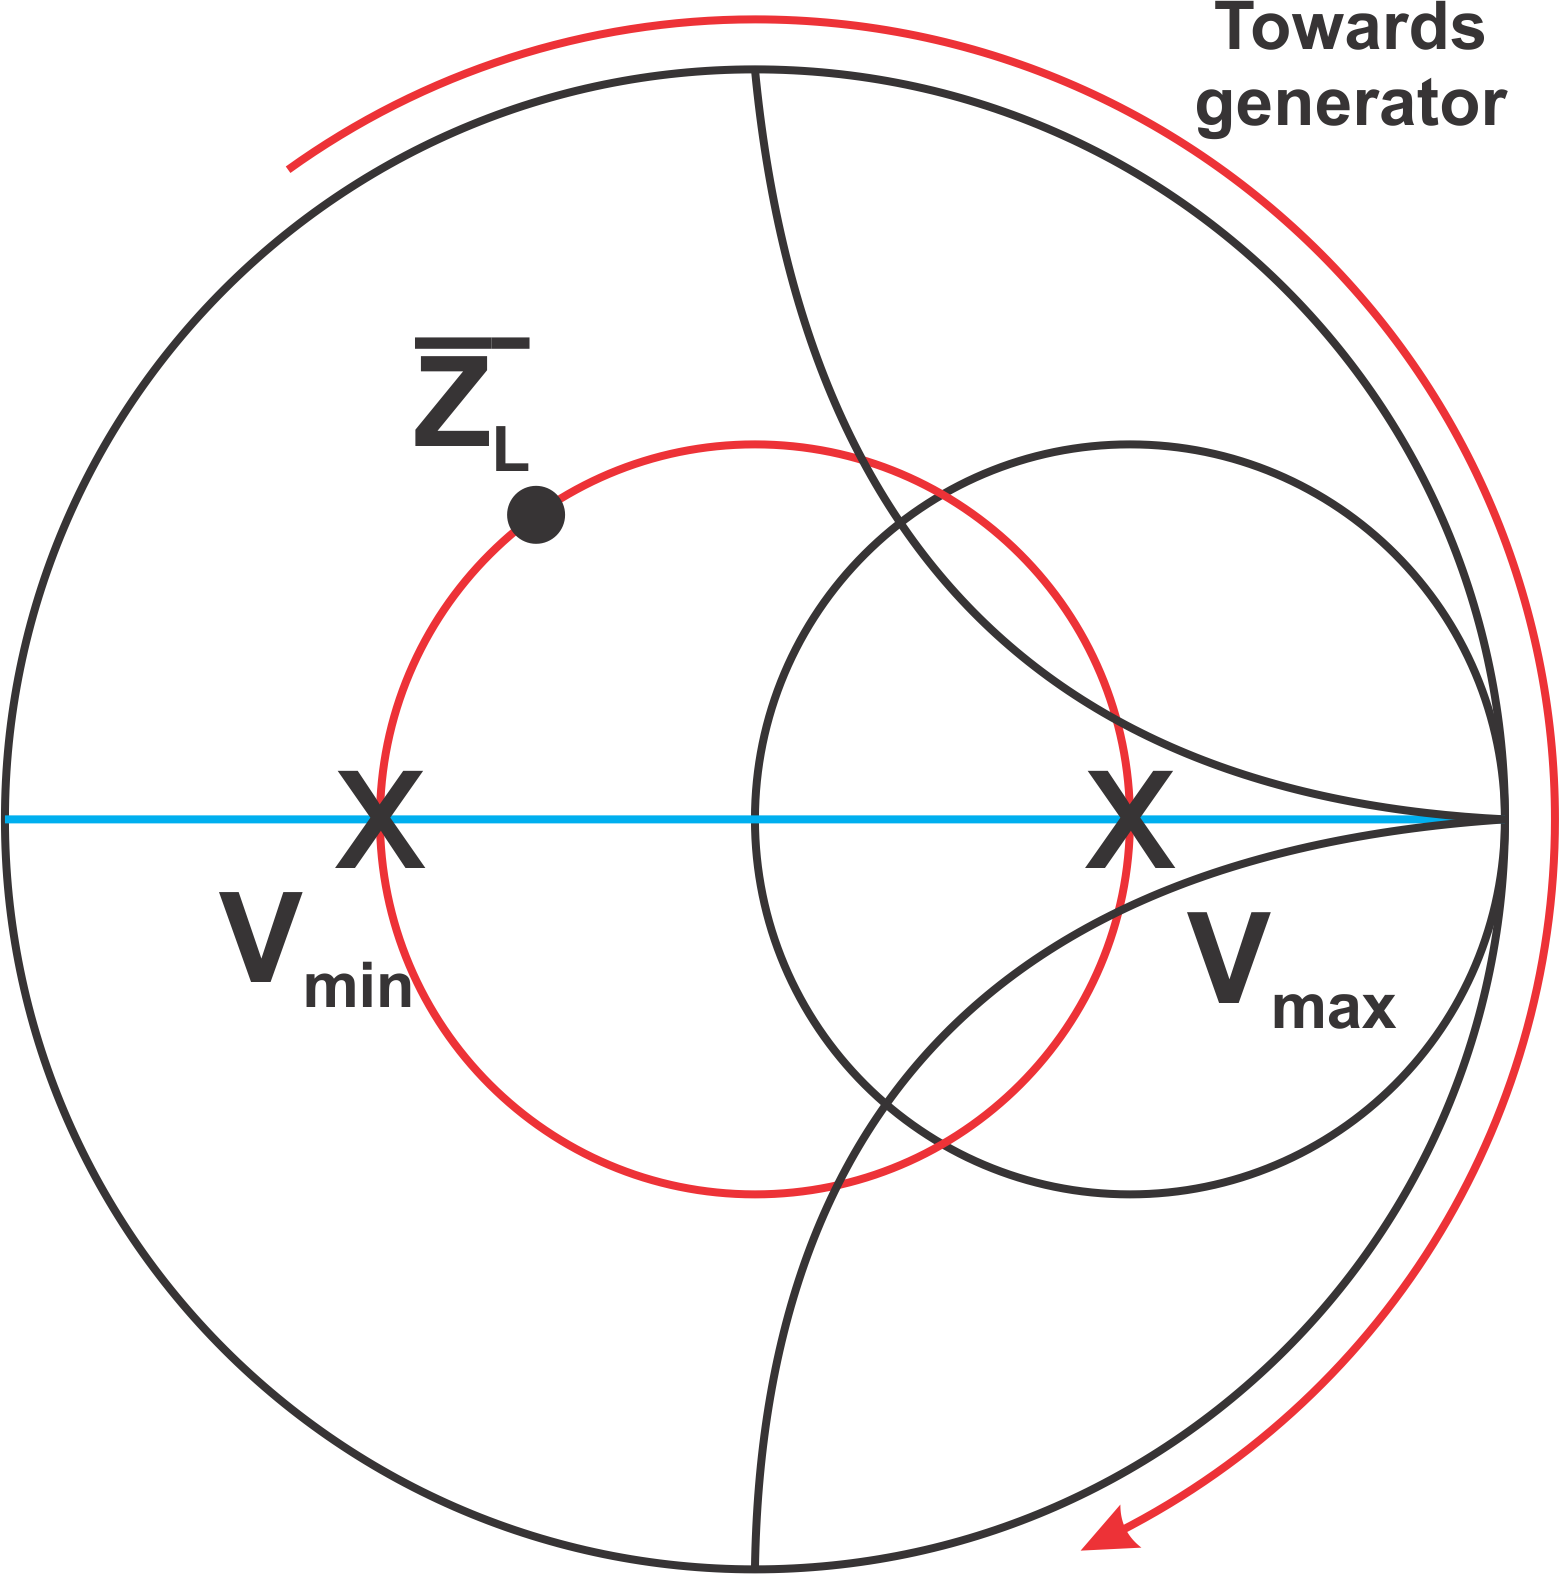
\includegraphics[scale=0.4]{./graphics/Group91}
\caption{A Smith chart representation of Inductive Load}
\end{figure}

\begin{figure}[h!]
\centering
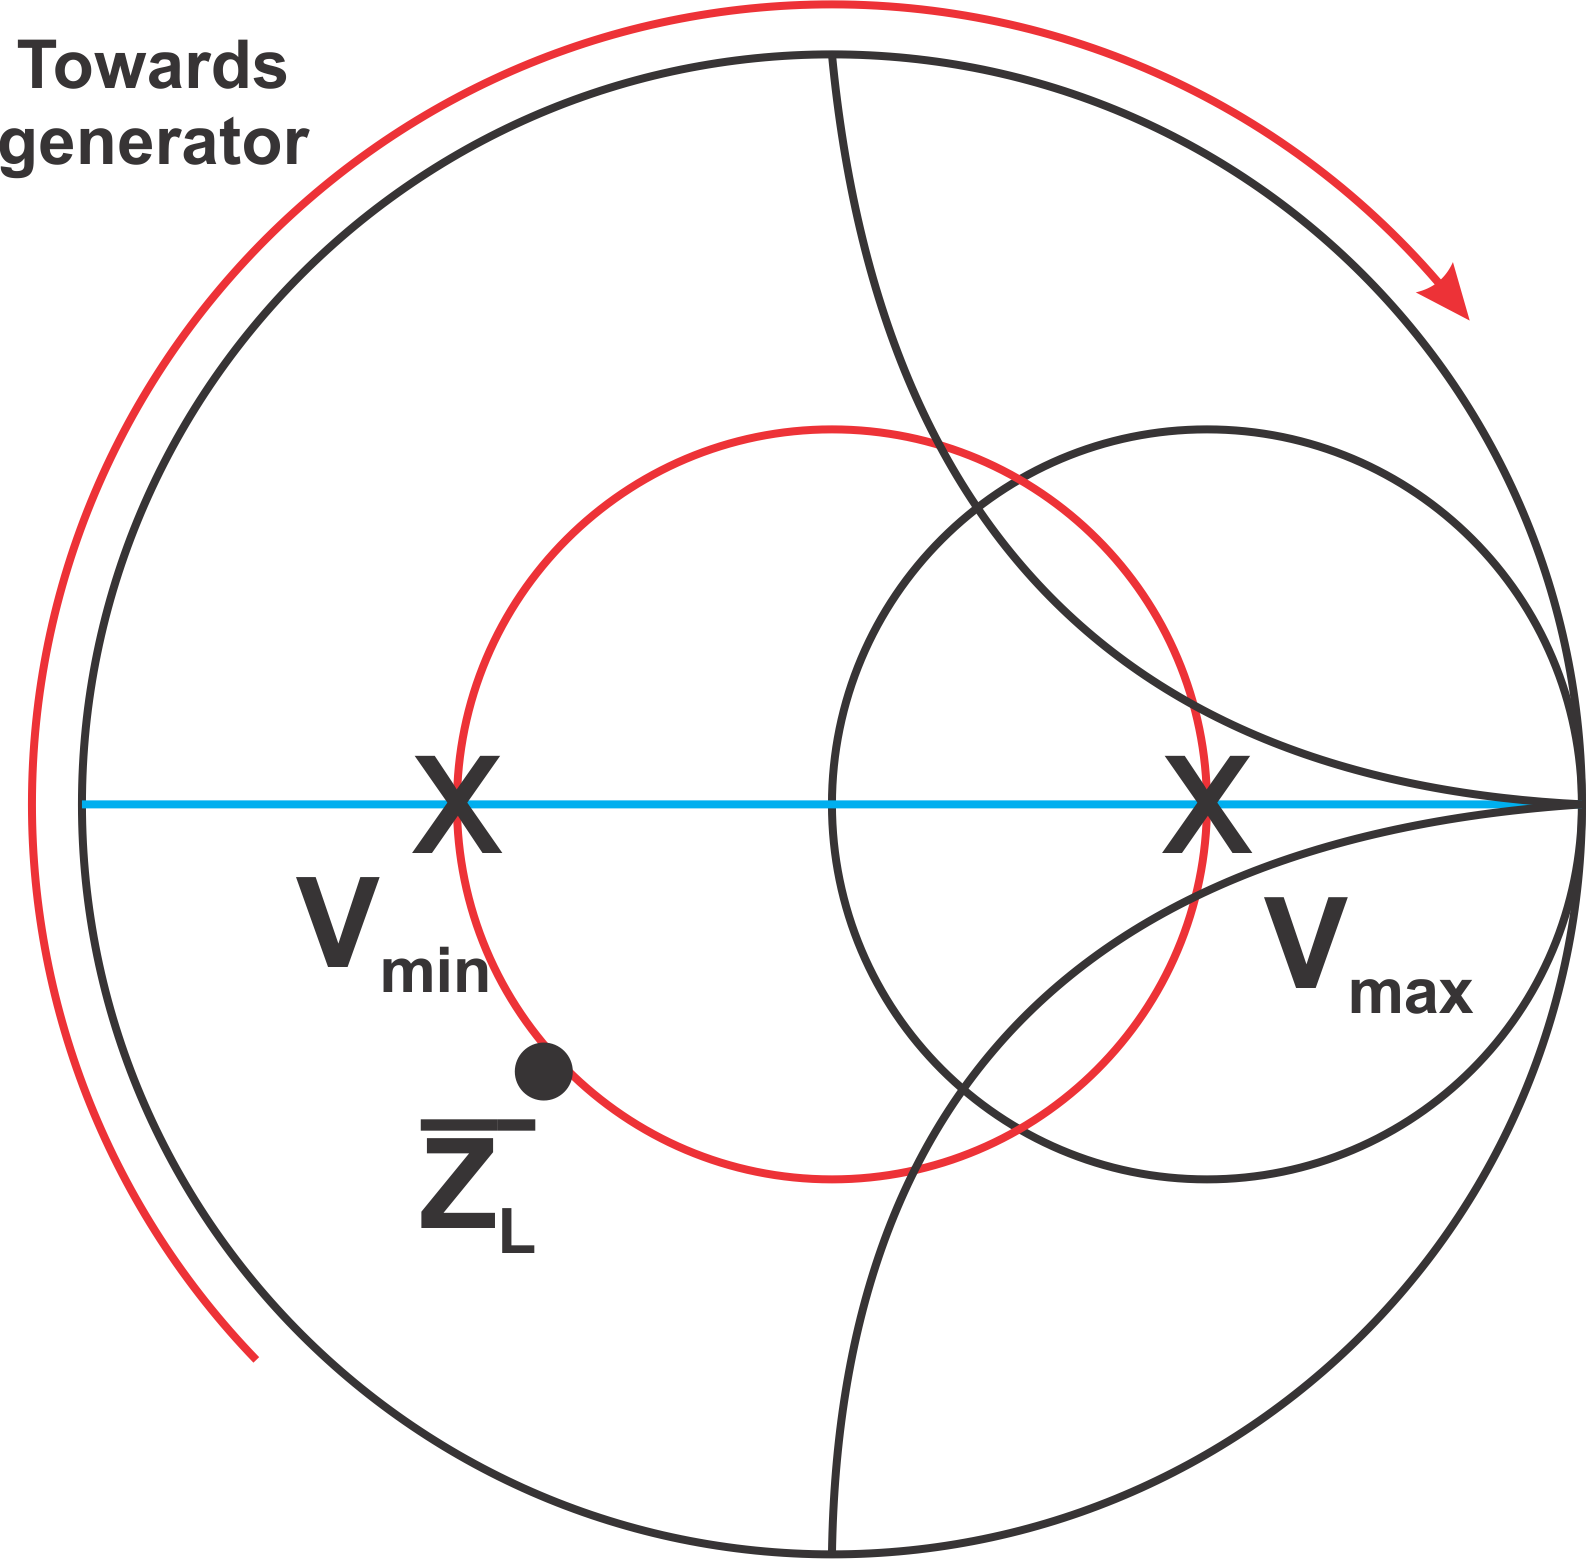
\includegraphics[scale=0.4]{./graphics/Group92}
\caption{A Smith chart representation of Capacitive Load}
\end{figure}From Figure 9.1, If we move from load towards the generator i.e. clockwise rotation, for the inductive load we encounter $V_{max}$ first before another $\frac{\lambda}{4}$ or $\pi rad$ movement to encounter ${V_{min}}$.\\
If we move from $\bar{Z_L}$ in clockwise direction for capacitive load, we encounter $V_{min}$ first before another $\frac{\lambda}{4}$ or $\pi rad$ movement to encounter $V_{max}$. $V_{min}\neq0$ means it is not a pure reactive load i.e $VSWR\neq\infty$\\
Now, let's analyze some standing wave graph and determine the type of load which they represent.
\begin{figure}[h!]
\centering
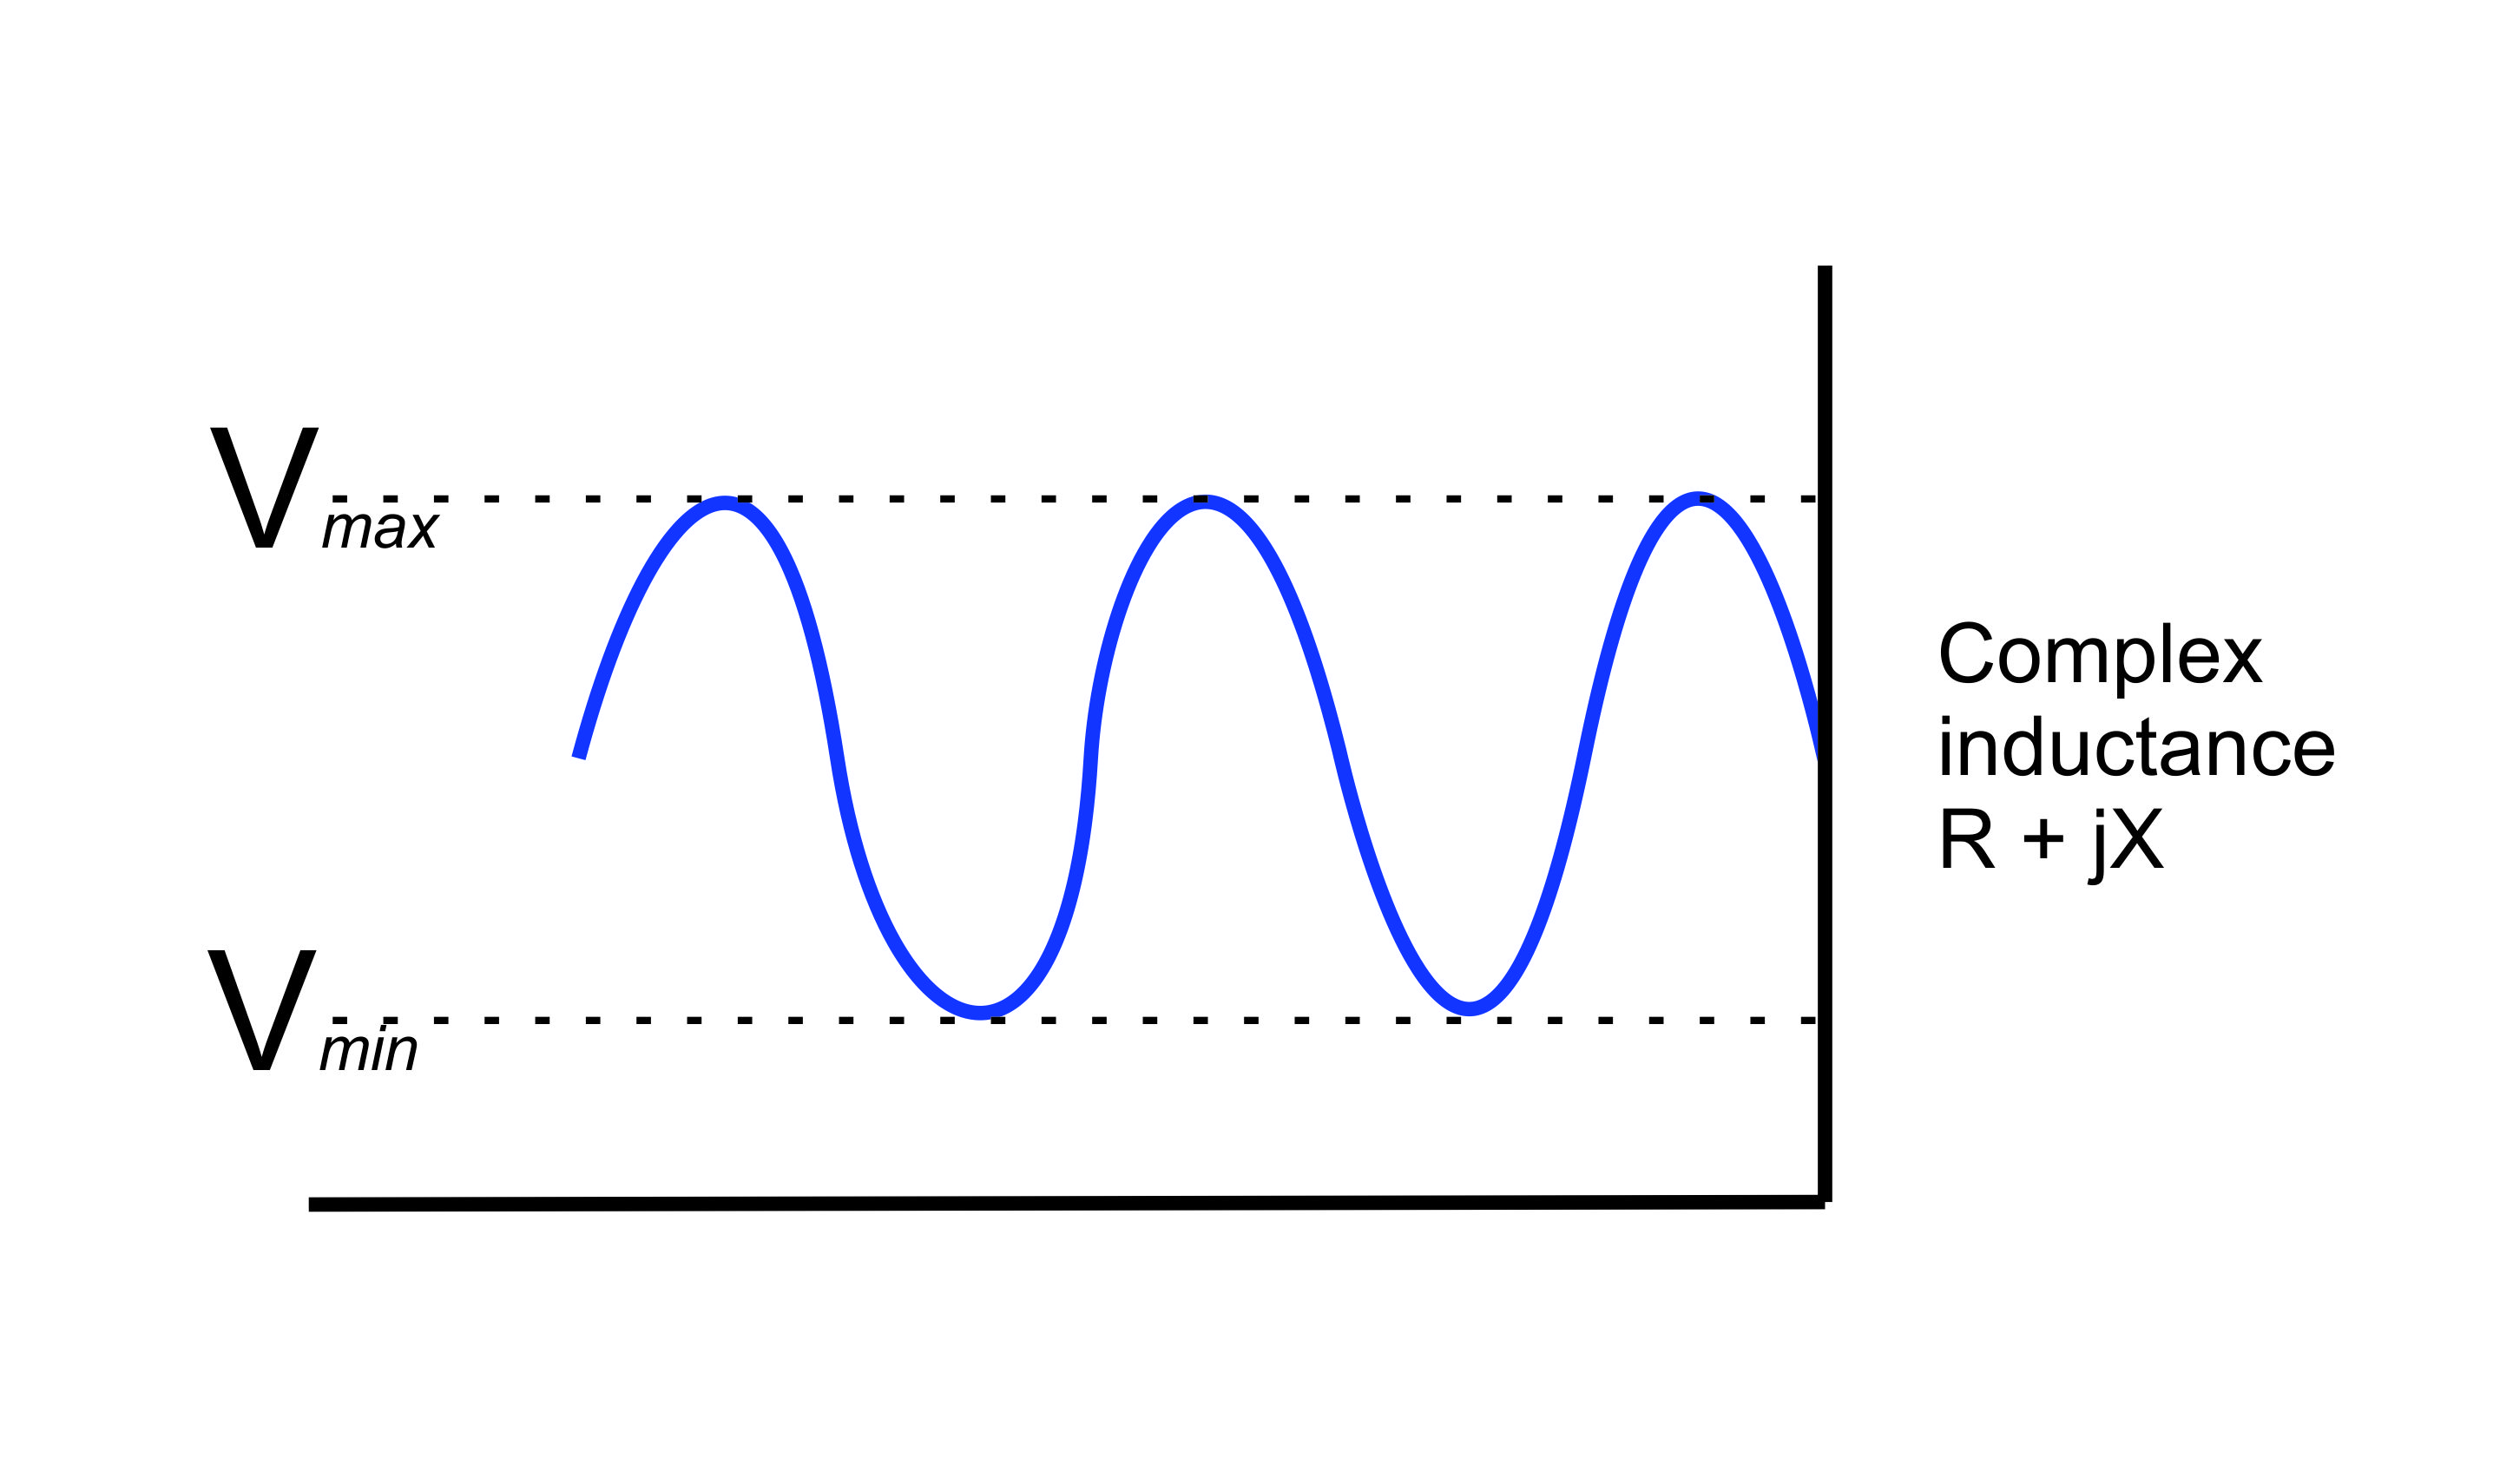
\includegraphics[scale=0.5]{./graphics/Group93}
\caption{Standing wave pattern variation of a complex Inductive load}
\end{figure}\\In Figure 9.3, the standing wave pattern moves from load towards the generator from right to left. It gets to a maximum first and its minimum is not zero as it does not touch the real axis. This indicates a complex inductance load which is similar to being on the upper half of the smith chart.\\
\begin{figure}[h!]
\centering
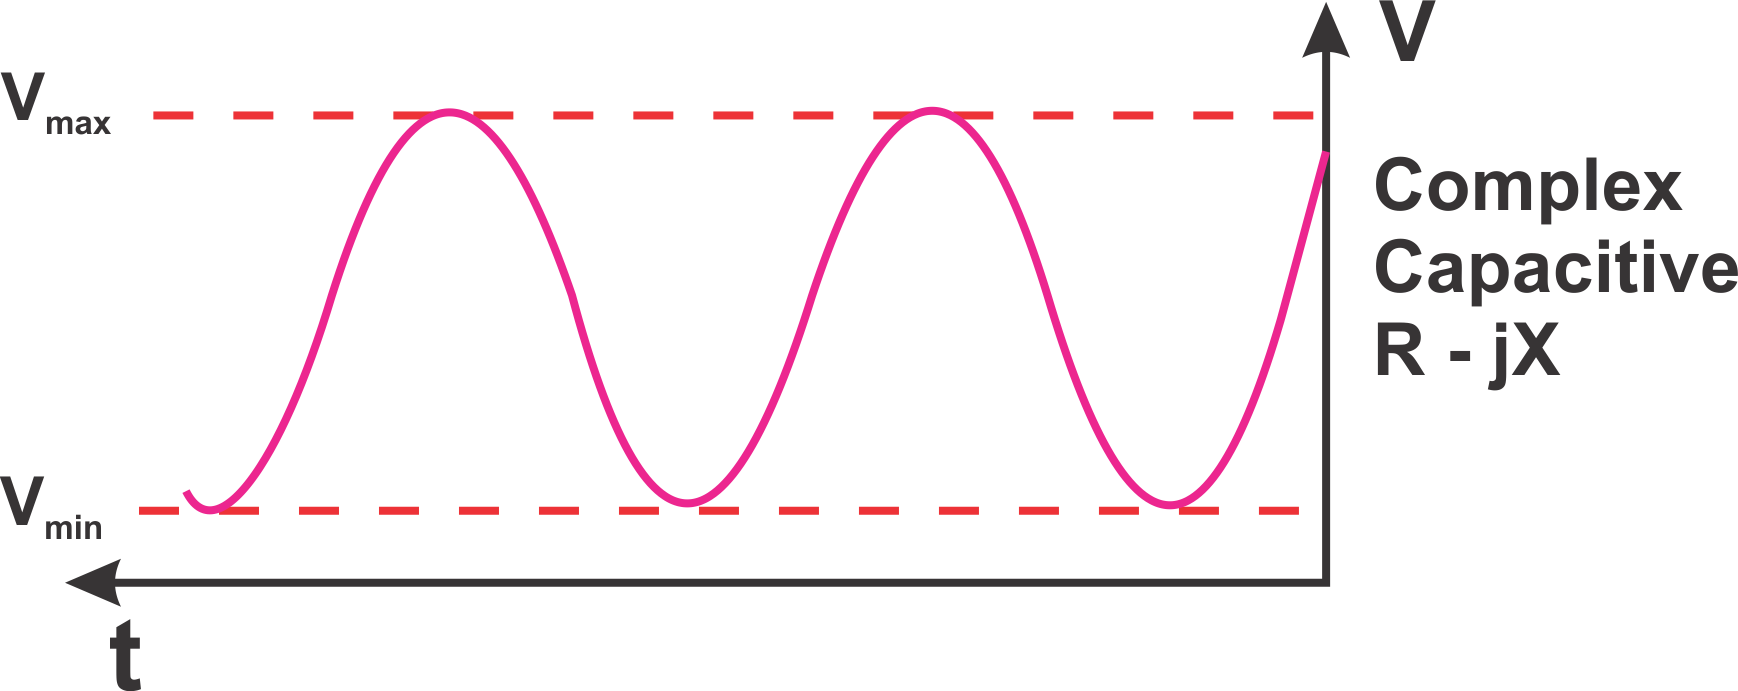
\includegraphics[scale=0.5]{./graphics/Group94}
\caption{Standing wave pattern variation of a complex Capacitive load}
\end{figure}\\In Figure 9.4, $V_{min}\neq0$ which means it is not purely reactive, we encounter $V_{min}$ first before $V_{max}$ indicating a complex capacitive load similarly to being on the lower half of the smith chart. The movement is towards the generator.\\

If the load is neither capacitive nor inductive, then it must lie on the real horizontal axis of the smith chart. So the location of the load itself will be at either the voltage minimum point or voltage maximum point.\\
\begin{figure}[h!]
\centering
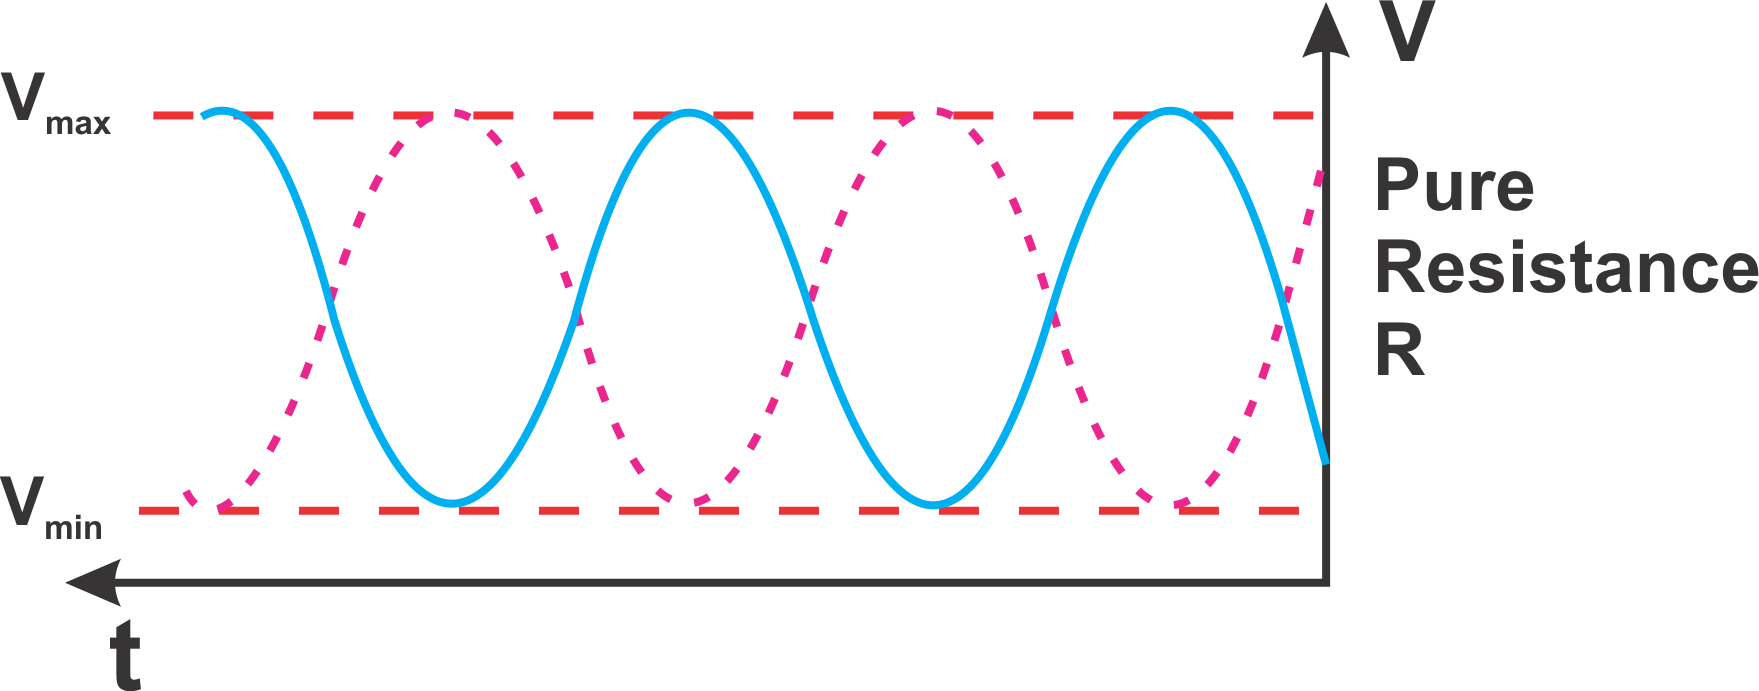
\includegraphics[scale=0.5]{./graphics/Group95}
\caption{Standing wave pattern variation of a pure Resistive load}
\end{figure}\\
If the load is purely reactive as in Figure 9.5. On the smith chart, the intersection of the VSWR circle on the real axis will be the location of the voltage maximum and minimum. So the load will have either the maximum or minimum voltage at the load end as shown in Figure 9.5. The thick curve has ${V_{max}}$ at load end meaning ${R>Zo}$. If ${V_{min}}$ is at load end, it means ${R<Z_o}$, ${Z_o}$ is the characteristics impedance.\\
\begin{figure}[h!]
\centering
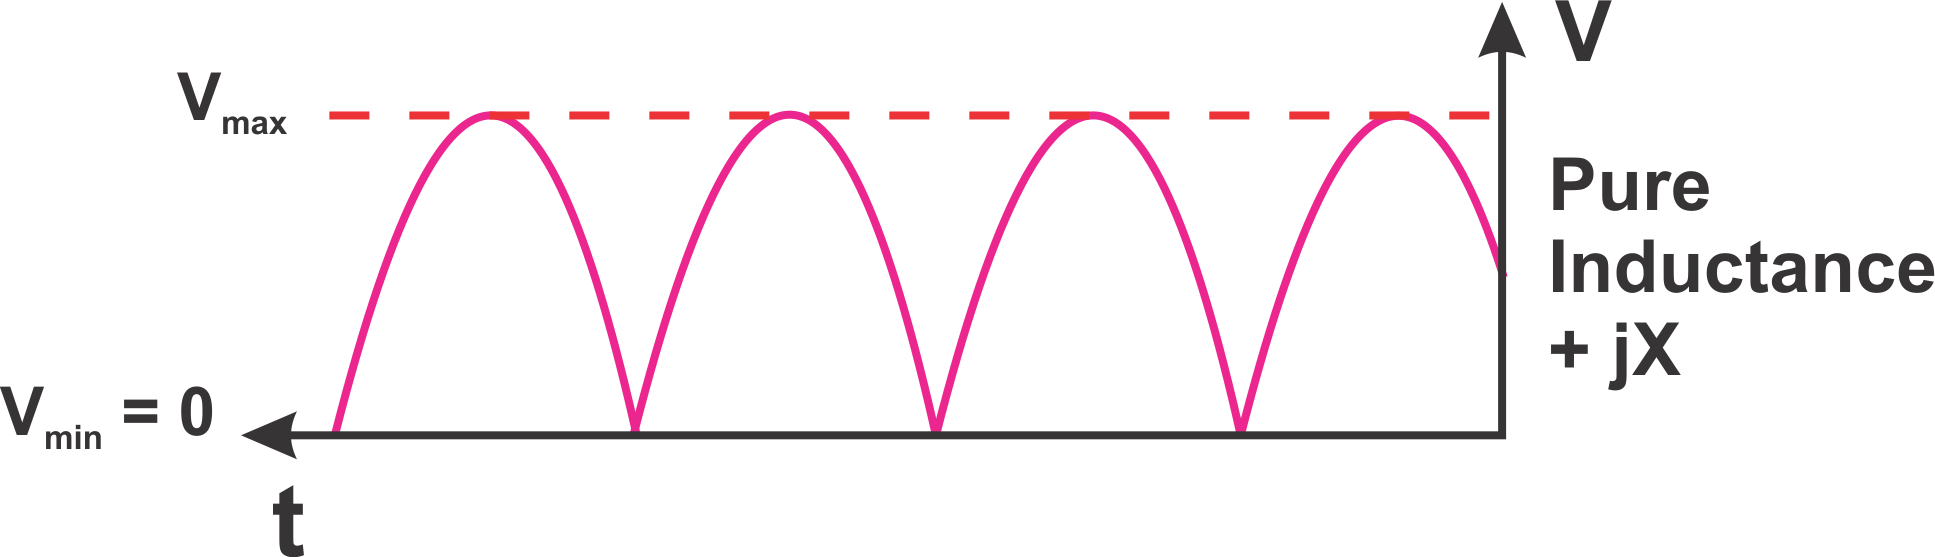
\includegraphics[scale=0.5]{./graphics/Group96}
\caption{Standing wave pattern variation of a pure Inductive load}
\end{figure}\\
In Figure 9.6, we observe that the voltage minimum is zero or it touches the horizontal axis i.e ${VSWR=\dfrac{V_{max}}{V_{min}}=\infty}$ as ${V_{min}=0}$. i.e purely reactive loads. As we move from the load end we meet ${V_{max}}$ first indicating it is purely inductive and lies on the upper half of the smith chart.\\
\begin{figure}[h!]
\centering
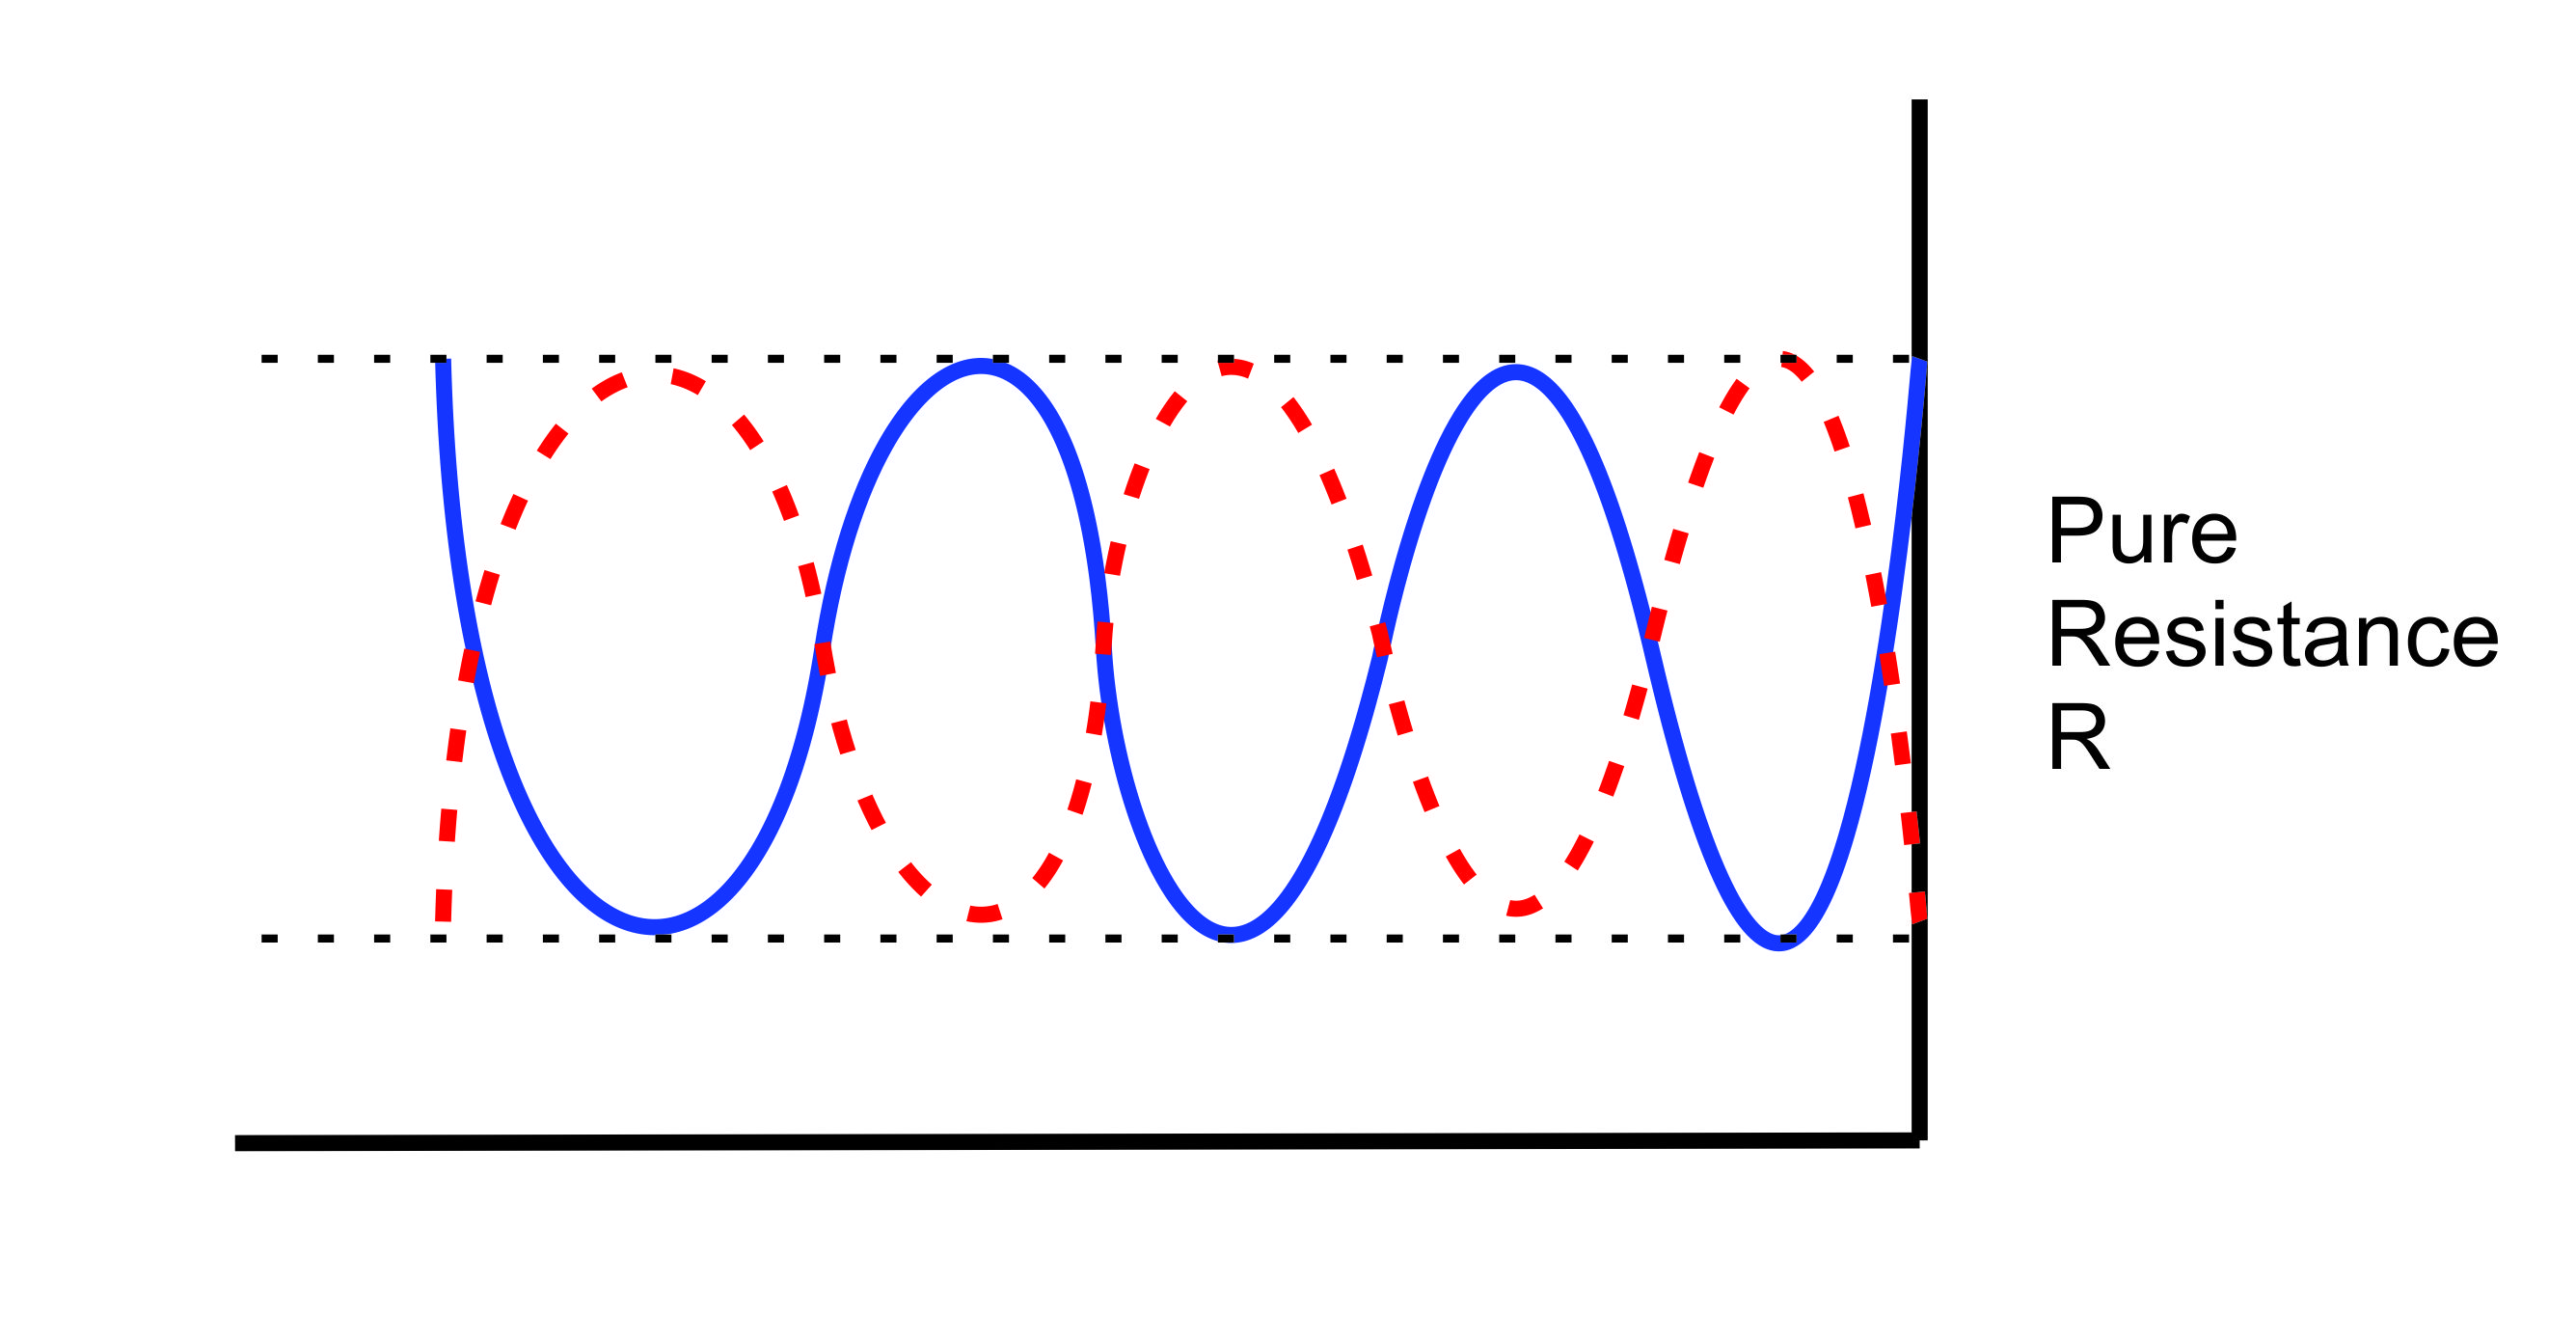
\includegraphics[scale=0.5]{./graphics/Group97}
\caption{Standing wave pattern variation of a pure Capacitive load}
\end{figure}\\
In Figure 9.7, the voltage minimum is also zero, but we encounter a minimum first as we go from the load end towards the generator indicating a purely capacitive load. So it lies in the lower half of the smith chart and $VSWR=\infty$.\\

So looking at the standing wave pattern, one can quickly identify the types of load because the information about the load is completely available from the standing wave pattern. Hence, ${V_{max}}$ and ${V_{min}}$ location and lowest value of ${V_{min}}$ which is related to VSWR can help us identity loads very quickly.\\

Now we solve some simple problems based on the theory we have developed from the transmission line.\\

\begin{center}
\textbf{PROBLEM 1}
\end{center}

A voltage wave at ${1GH}z$ is traveling on a transmission line in ${+x}$ direction. The primary constants of the line are ${R=0.5\Omega/m}$, ${L=0.2\mu H/m}$, ${G=0.1\upsilon/m}$, ${C=100pF/m}$. Calculate the attenuation constant in ${nepers/m}$ and ${dB/m}$. If the voltage of the forward traveling wave at ${t=0}$ and ${x=0}$ ${v}=0.866V$. Find the voltage at ${x=1m}$ and time ${t=100nsec}$. What is the peak voltage at ${x=1m?}$ Take initial phase as ${30^0}$.


\begin{center}
\textbf{Solution to Problem 1}
\end{center}
$ \omega = 2\pi\times 10^{9} $ rad/sec\\
Propagation constant $\gamma = \sqrt{(R + \jmath\omega L)(G + \jmath\omega C)}$
\begin{dmath*}
\gamma=\\
 \sqrt{(0.5 + \jmath( 2\pi\times 10^{9} \times 0.2\times 10^{-6}))(0.1 + \jmath (2\pi\times 10{9} \times 10^{-12}))} \quad
\end{dmath*}

$ = 2.23 + \jmath 28.2$ per metre\\ 
$\gamma = \alpha + \jmath\beta$\\
where $\alpha$ = Attenuation constant and $\beta$ = Phase constant\\

$\Rightarrow \alpha$ = 2.23 \emph{Nepers/m} and $\beta$ = 28.2 \emph{rad/m}\\
but 1 Nepers/m = 8.68\emph{dB/m}\\
$\Rightarrow$ 2.23 \emph{Nepers/m} = 2.23$\times$8.68= 19.36 \emph{dB/m}\\\\
Now to find $V_{(x,t)}$, we shall express $V_{(x,t)}$ in general as \\\\
$V_{(x,t)} = (V^{+}e^{-\gamma x} + V^{-}e^{+\gamma x})e^{j\omega t}$ for forward and backward wave.\\\\
Since we are dealing with only forward wave $ V^{-} = 0 $.\\\\
$V_{(x,t)} = V^{+}e^{-\gamma x}e^{j\omega t}$\\\\
$V_{(x,t)} = Re({V^{+}e^{-(\alpha +j\beta)x}e^{j\omega t}})$\\\\
$V_{(x,t)} = Re({V^{+}e^{-\alpha x}e^{-j\beta x}e^{j\omega t}})$\\\\
$V_{(x,t)} = Re({V^{+}e^{-\alpha x}e^{j(\omega t - \beta x)}})$\\\\The real or imaginary part is sufficient to characterize the sinusoidal variation with time, ${e^{j\omega t}}$ is very general.\\\\
${V^+}$ has an amplitude and initial phase. Hence, it is a complex quality expressed as $ V^{+} = |V^{+}|e^{\jmath\phi} $, $ |V^{+}| =$ Amplitude and $ \phi =$ initial phase\\\\
$V_{(x,t)} = Re({|V^{+}|e^{-\alpha x}e^{j\phi}e^{j(\omega t - \beta x)}})$\\\\
$V_{(x,t)} = Re({|V^{+}|e^{-\alpha x}e^{j(\phi+\omega t - \beta x)}})$\\\\
$V_{(x,t)} = Re({|V^{+}|e^{-2.23x}e^{(\phi+2\pi10^9t-28.2x)}})$\\\\
At $ x = 0, t = 0, \quad \quad V(x,t) = 8.66V $ then at these values\\\\ 
$8.66 = Re({|V^{+}|e^{-0}e^{j(\phi+0-0)}}) \quad = Re({|V^+|}e^{j\phi})$\\\\
$Re({V^{+}e^{j\phi}}) = Re({V^{+}{cos\phi}} + {jV^{+}{sin\phi}}) = |V^{+}|{cos\phi}$\\\\
$Re({|V^{+}|e^{-\alpha x}e^{j(\phi+\omega t - \beta x)}}) = ({|V^{+}|e^{-\alpha x}cos{(\phi+\omega t - \beta x)}})$\\\\
$8.66 = {|V^+|{cos\phi}} \quad$ at $ \phi = 30^{o} $\\\\
$8.66 = {|V^+|{cos30}}$\\\\
$8.66 = {|V^+|{0.866}}$\\\\
$\frac{8.66}{0.866} = {|V^+|}$\\\\
${|V^{+}| = 10V}$\\\\
Hence, the complete expression is\\
$V_({x,t}) = 10e^{-2.23x} cos({\dfrac{\pi}{6} + 2\pi\times10^9t - 28.2x})$\\\\
To find voltage at x=1m and t=100nsec, we have\\
$V_({1,100nsec}) = 10e^{-2.23} cos({\dfrac{\pi}{6} + 2\pi\times10^9\times100\times10^{-9} - 28.2\times1})$\\\\
$V_({1,100nsec}) = -0.88V$\\\\
$V_({x,t}) = 10e^{-2.23x} cos({\dfrac{\pi}{6} + 2\pi\times10^9t - 28.2x})$\\\\
The peak value at x = 1m is given thus\\\\
$V_({1,t}) = 10e^{-2.23(1)} cos({\dfrac{\pi}{6} + 2\pi\times10^9t - 28.2(1)})$\\\\
Peak value happens when $cos({\dfrac{\pi}{6} + 2\pi\times10^9t - 28.2(1)}) = 1$\\\\
$ V_{(1,t)_{max}} = 10e^{-2.23} = 1.07528V $\\\\
This is one of the simplest problem of a Transmission Line, where the primary constants are given and voltage at some instant of time and location is also given. We are then asked to find out the voltage at some other location and at some other instant of time.\\
\begin{center}
\textbf{PROBLEM 2}
\end{center}
If the wave in the previous example is traveling in the negative ${x}$ direction, with all other things same. Find the instantaneous  voltage at the same time and at the same location.\\
\begin{center}
\textbf{SOLUTION}
\end{center}
For the wave travelling in the negative direction, we have\\
$V_{(x,t)} = Re(V^{-}e^{\gamma x}e^{j\omega t})$ for backward wave.\\\\
$Re({V^{-}e^{\alpha x}e^{j\beta x}e^{j\omega t}}) = {|V^{-}|e^{\alpha x}cos{(\phi+\omega t + \beta x)}}$\\\\
At ${t=0, x=0, V=8.66}$, then\\\\
${8.66} = {|V^{-}|}e^{0} cos({\phi + 0 + 0})$\\\\
$8.66 = {|V^-|{cos\phi}} \quad$ at $ \phi = 30^{o} $\\\\
$8.66 = {|V^-|{cos30}}$\\\\
$8.66 = {|V^-|{0.866}}$\\\\
$\frac{8.66}{0.866} = {|V^-|}$\\\\
${|V^{-}|} = 10V$\\\\
$V_({x,t}) = 10e^{2.23x} cos({\dfrac{\pi}{6} + 2\pi\times10^9t + 28.2x})$\\\\
At ${t=100nsec}$ and ${x=1m}$\\\\
$V_({x,t}) = 10e^{2.23} cos({\dfrac{\pi}{6} + 2\pi\times10^9\times100\times10^{-9} + 28.2})\\\\
= -83.7701V$\\\\
\begin{figure}[h!]
\centering
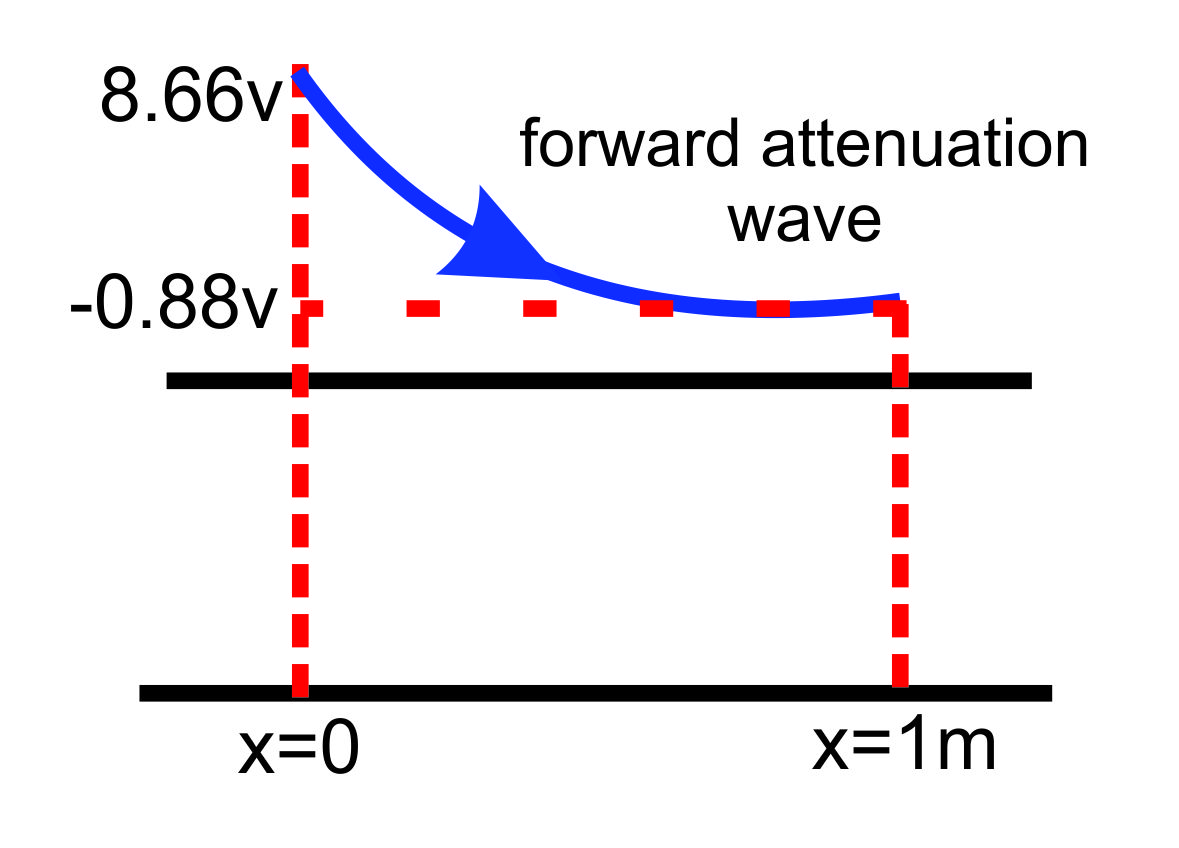
\includegraphics[scale=0.5]{./graphics/Group98}
\caption{Diagram for Problem 2}
\end{figure}
So what we note here is, if we look at the transmission line with ${x=0}$ and ${x=1m}$. If the wave travels in forward direction, then the wave will attenuate in the direction of propagation. The variation is from ${8.66V}$ to ${-0.88V}$. In the backward direction, the wave will attenuate in the reverse direction so it has to  have a higher amplitude at ${x=1m}$ and ${t=100nsec}$ from were it attenuates from ${-83.7701V}$ to ${8.66V}$ in the other direction. The direction of propagation of the wave is very important.\\
\begin{center}
\textbf{PROBLEM 3}
\end{center}
A transmision line has $L = 0.25muH/m$, $C=100pF/m$ and ${G=0}$. What should be the value of ${R}$ for the line so that the line can be travelled as a low loss line? The frequency of operation is ${100MHz}$.\\
\begin{center}
\textbf{SOLUTION}
\end{center}
For low loss line ${\alpha\ll\beta}$ say ${100\alpha=\beta}$ at 1 percent of ${\beta}$ value\\\\
${\beta=\omega\sqrt{LC}} = {2\pi\times100\times10^6\sqrt{0.25\times10^{-6}\times100\times10^{-12}}}$\\\\
${\beta=2\pi\times100\times10^6\times5\times10^{-9}}$\\\\
${\beta=\pi}$\\\\			${\alpha={\dfrac{1}{2}}(R\sqrt{\dfrac{C}{L}}+G\sqrt{\dfrac{L}{C}})}$\\\\
G = 0, So that:\\\\
${\alpha={\frac{R}{2}}\sqrt{\frac{C}{L}}}$\\\\
${\alpha=\frac{R}{2}\sqrt{\frac{100\times10^{-12}}{0.25\times10^{-6}}}}$\\\\
${\alpha=\frac{R}{2}\sqrt{\frac{1}{2500}}}$\\\\
${\alpha=\frac{R}{2}\times\frac{1}{50}}$\\\\
${\alpha=\frac{R}{100}}$\\\\
Remember 
${\alpha = \frac{\beta}{100}}$\\\\
Since ${\beta = \pi}$\\\\
${\alpha = \frac{\beta}{100} = \frac{\pi}{100} = \frac{R}{100}}$\\\\
${R = \pi\Omega/m}$\\\\ 
So for this transmission line taking a resistance of ${3\Omega /m}$. It can be treated as a low loss transmission line. If ${R>\pi}$ say ${4\Omega}$, it is no more a low loss transmission line and it slowly become a lossy transmission line. When ${R}$ increases to the point that ${\alpha\approx\beta}$, then the line becomes extremely lossy.\newpage

\begin{center}
\textbf{SUMMARY}
\end{center}
So in this section, we have shown how to identify the load by looking at standing wave patterns. Next we solved some simple problems for transmission line based on voltage equations which we have derived for the transmission line. Next we go to applications of transmission line since we make use of sections of transmission line in realizing various circuit elements in high frequency circuits.\\		
